% Created 2021-09-12 Sun 22:48
% Intended LaTeX compiler: xelatex
\documentclass[letterpaper]{article}
\usepackage{graphicx}
\usepackage{grffile}
\usepackage{longtable}
\usepackage{wrapfig}
\usepackage{rotating}
\usepackage[normalem]{ulem}
\usepackage{amsmath}
\usepackage{textcomp}
\usepackage{amssymb}
\usepackage{capt-of}
\usepackage{hyperref}
\usepackage[margin=1in]{geometry}
\usepackage{fontspec}
\usepackage{indentfirst}
\setmainfont[ItalicFont = LiberationSans-Italic, BoldFont = LiberationSans-Bold, BoldItalicFont = LiberationSans-BoldItalic]{LiberationSans}
\newfontfamily\NHLight[ItalicFont = LiberationSansNarrow-Italic, BoldFont       = LiberationSansNarrow-Bold, BoldItalicFont = LiberationSansNarrow-BoldItalic]{LiberationSansNarrow}
\newcommand\textrmlf[1]{{\NHLight#1}}
\newcommand\textitlf[1]{{\NHLight\itshape#1}}
\let\textbflf\textrm
\newcommand\textulf[1]{{\NHLight\bfseries#1}}
\newcommand\textuitlf[1]{{\NHLight\bfseries\itshape#1}}
\usepackage{fancyhdr}
\pagestyle{fancy}
\usepackage{titlesec}
\usepackage{titling}
\makeatletter
\lhead{\textbf{\@title}}
\makeatother
\rhead{\textrmlf{Compiled} \today}
\lfoot{\theauthor\ \textbullet \ \textbf{2021-2022}}
\cfoot{}
\rfoot{\textrmlf{Page} \thepage}
\titleformat{\section} {\Large} {\textrmlf{\thesection} {|}} {0.3em} {\textbf}
\titleformat{\subsection} {\large} {\textrmlf{\thesubsection} {|}} {0.2em} {\textbf}
\titleformat{\subsubsection} {\large} {\textrmlf{\thesubsubsection} {|}} {0.1em} {\textbf}
\setlength{\parskip}{0.45em}
\renewcommand\maketitle{}
\author{Houjun Liu}
\date{\today}
\title{Proteins}
\hypersetup{
 pdfauthor={Houjun Liu},
 pdftitle={Proteins},
 pdfkeywords={},
 pdfsubject={},
 pdfcreator={Emacs 28.0.50 (Org mode 9.4.4)}, 
 pdflang={English}}
\begin{document}

\maketitle


\section{Proteins}
\label{sec:orgc191180}
All cell uses \emph{rybozome} to force
\href{KBhBIO101AminoAcids.org}{KBhBIO101AminoAcids} together to make
proteins. And yes, if you have a high energy source that would not
require ATP from itself (make life from not life), you could get
proteans to fold.

\subsection{Protean Shapes}
\label{sec:org143a3aa}
Proteins, when unfolded, is a long chain of amino acids. When they are
folded in different configurations, you get a working protean.

\noindent\rule{\textwidth}{0.5pt}

The functions of proteins are varied because the primary sequence can be
varied, effectively building any shape protein to do its specific
function

\textbf{Form = function} is the idea that the shape or form a protein takes
through the combination of primary, secondary, tertiary, or quaternary
structure determines how it will then function. Any changes to the
structure will have some impact on its function and the more the
structure is affected the more the function is likely to impacted.

Functions => defense, movement, structure, transport, cell to cell
signaling, etc.

\noindent\rule{\textwidth}{0.5pt}

"The Protean Folding Problem" => can we find the fold of the protean
just by the unfolded amino acids?

\subsubsection{Protean primary structure}
\label{sec:org628a205}
The linear order of amino acids --- staring from the amino terminus (N,
exposes the \emph{Amine} end) and moving to carbonxy terminusi (C, exposes
the \emph{Carboxy} terminus).

Average protean is about 300 amino acids long.

\subsubsection{Protean secondary structure}
\label{sec:org61453bb}
Folding a protean without concern to the amino acid side chains. The
folding is only concerned with being stabilized with dipole attraction
to hydrogen.

Two main secondary structures: the alpha helix and beta sheet.

\begin{figure}[htbp]
\centering
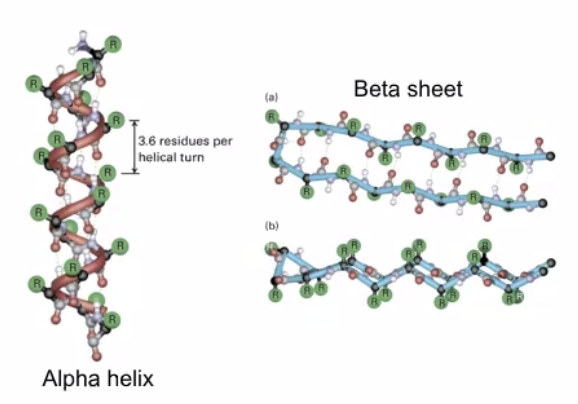
\includegraphics[width=.9\linewidth]{/Users/houliu/Documents/School Work/2020-2021/KnowledgeBase/2020BIO101/Screen Shot 2020-09-21 at 3.15.49 PM.png}
\caption{Screen Shot 2020-09-21 at 3.15.49 PM.png}
\end{figure}

*No ionic attractions between backbone because after the dehydration
reaction (polymerization), the positive and negative of the two ends of
the backbone of the amino acid is combined to cancel out the charge*

Proline (p) is a little weird: Side chain bonded with the H2N+ as well
as the carbon => "the helix breaker": most likely cause a bend instead
of a structured area due to its unusual circular bonding.

\subsubsection{Protein Tertiary Structure}
\label{sec:orgd1d1712}
Bonds in the 3D Structures

\begin{itemize}
\item Non-polar sidechains: Vandervaull's Forces (a.k.a LDF)
\item Ionic sidechains: what bonds do you think?
\item Disulfide bonds: cysteine animo acids will bond their sulfur together
\item Polar sidechains: hydrogen bonds
\end{itemize}

All of these bonds, together, makes the 3D geometry of the protean.

\textbf{Proteins fold in order of attraction strength.}

\begin{itemize}
\item Proteas "whiggle" --- brounian motion
\item This is also a part of the difficulty in folding protean
\end{itemize}

\subsubsection{Protein Quaternary Structure}
\label{sec:org2f4510d}
Exists only for certain proteins which independently locks together.

Hemoglobin does this! It contains multiple sets of side chains that
needs folding once again.

\subsection{Shooting images of proteins}
\label{sec:orgf6ed8de}
\begin{itemize}
\item NMR spectroscopy
\item X-rays
\end{itemize}

\#flo \#disorganized

\subsection{Enzymes}
\label{sec:org31cb1f4}
A specific type of proteins that's\ldots{} kinda fun!
\href{KBhBIO101Enzymes.org}{KBhBIO101Enzymes}
\end{document}
